% This is part of Un soupçon de mathématique sans être agressif pour autant
% Copyright (c) 2015
%   Laurent Claessens
% See the file fdl-1.3.txt for copying conditions.

\begin{exercice}[\cite{NRHooXFvgpp4}]\label{exo2smath-0061}

    \begin{multicols}{2}

        L'instrument de Gerbert est constitué de deux bâtons $[AB]$ et $[ED]$ perpendiculaires tels que $AD = ED$.  Soit $S$ le sommet de l'arbre. Pour mesurer sa hauteur, il faut se placer de telle sorte que les points $S$, $A$ et $E$ soient alignés. Ses mesures sont : \( AD=\SI{0.4}{\meter}\) et \( AB=\SI{0.5}{\meter}\).

        Le point \( S\) est inaccessibles, c'est à dire que les distances \( AS\), \( SP\), etc. ne peuvent pas être mesurées.

        Quelles mesures et calculs doit-on faire pour savoir la hauteur de l'arbre ?

\columnbreak

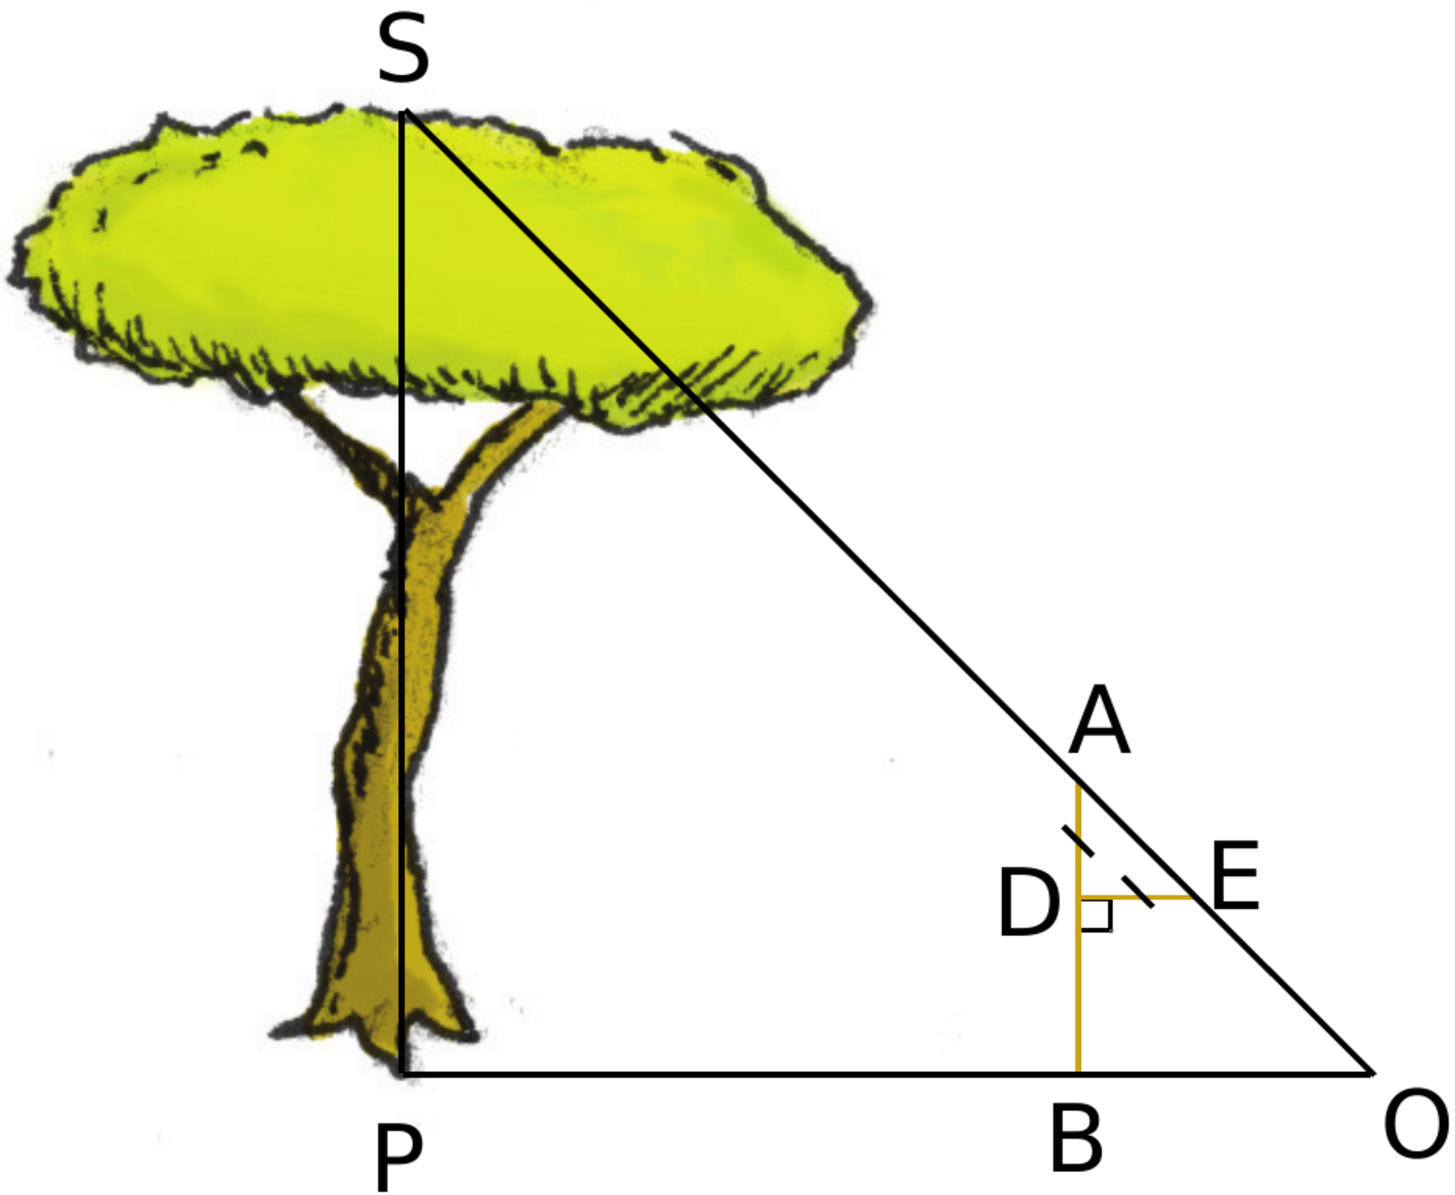
\includegraphics[height=4.5cm]{arbre.pdf}


    \end{multicols}

\corrref{2smath-0061}
\end{exercice}
